\section{Multi-digit MNIST Octal-division Task}
\label{sec:task}

The multi-digit MNIST octal-division task can be formulated as follows: given two lists of MNIST images representing multi-digit octal numbers, we want to perform the division between the two numbers. We constrain the problem assuming that the second number is an integer divisor of the first. Moreover, we generate the training set in such a way that it contains only single-digit numbers in order to show how the program can be extended to multi-digit numbers without being explicitly trained on them.
% With this task, we can test the 
% while the test set contains multi-digit numbers. In this way, the framework is able to show the high-level reasoning capabilities

The main goal in the DeepProbLog program is to define the predicate \texttt{division(X,Y,Z)}, where X and Y are lists of images of handwritten digits from the MNIST dataset that represent two base-8 numbers and Z is the base-8 number corresponding to the result of the division between X and Y. While such a predicate can be learned directly by a standard neural classifier, such an approach cannot incorporate background knowledge such as the definition of the octal division between two numbers.
%  and as a consequence requires more iterations to converge, multi-digit numbers in the test set, larger test set. % TODO

\begin{figure}[ht]
\centerline{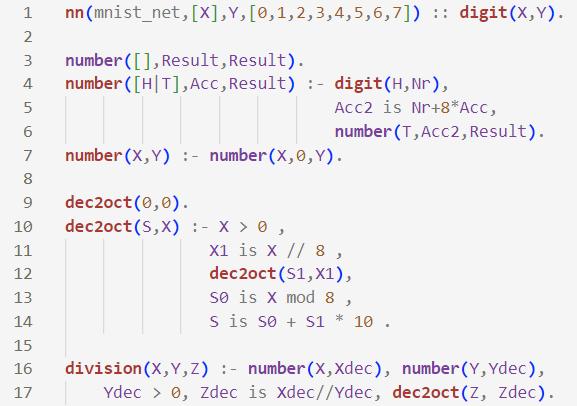
\includegraphics[scale=0.7]{problog_model.png}}
\caption{The DeepProbLog program.}
\label{fig:program}
\end{figure}

The DeepProbLog program implemented to solve the task is shown in Fig. \ref{fig:program}. The program specifies the neural annotated disjunction

\begin{equation}
    nn(mnist\_net,[X],Y,[0,1,2,3,4,5,6,7]) :: digit(X,Y).
\end{equation}

where $nn$ is a reserved functor, $mnist\_net$ is a neural network that classifies MNIST digits defining a probability distribution over the domain ${1,2,3,4,5,6,7}$ 
% composed of 8 elements since the input is an image of a base-8 digit, 
and $digit$ is the corresponding neural predicate. The output layer of the network that feeds the $digit$ neural predicate should be normalized in order to get proper probability values. In general, the neural network, apart from the output layer, could be of any kind, e.g., a recurrent network for sequence processing or a convolutional network for image processing. We decided to implement the standard convolutional network used for MNIST images since it is the more suitable neural network for MNIST images. % TODO: reference to nn

% The program contains also some rules, as shown in Fig. \ref{fig:program}. These rules permit to obtain the base-8 number from the input list of MNIST digits, convert it to a decimal number, apply the standard Prolog operator for the integer division between decimal numbers, and finally convert back the result to an octal number.

The DeepProbLog program proceeds as follows: given a training example composed of two lists of MNIST images and the result of the division in base-8, first we need to obtain the dividend and divisor from the list of images. This is done passing the images to the neural network and building the base-10 numbers from the single digits. Then the division can be calculated applying the standard Prolog operator for the integer division between decimal numbers and the result converted back to a base-8 number. The learning process can be applied based on the supervised label and on the obtained result.


% a neural predicate \texttt{digit} which maps an image of a digit $I_D$ to the corresponding natural number $N_D$.

% The ProbLog program is composed by the neural predicate \texttt{digit(x,y)} that given an image.


\subsection{Training and test sets}
Starting from the MNIST dataset we constructed the training and test sets as follows. The training set is composed of pair of images that represent single-digit base-8 numbers and the test set is composed of two lists of images that represent three-digit base-8 numbers. In both cases, the second number is a divisor of the first one. % TODO: not always 3 digits
After removing the images representing digit 8 or 9 from the MNIST training and test sets, the algorithm proceeds constructing a random number $n_1$. Then, a random divisor $n_2$ is constructed: we select a random number in the range $[1,n_1]$ and we select the nearest number that is a divisor of $n_1$. The images used to construct the two numbers are removed from the MNIST dataset. Proceeding in this way until no more pairs can be constructed, we managed to generate a training set made of $22958$ pairs and a test set made of $1462$ pairs. We fixed the random seed to obtain always the same dataset. In this way, there are no repeated images in the training and test sets but not all the MNIST images will be used: we used $45916$ of the available $48200$ training images of MNIST ($95.26\%$) and $7835$ of the available $8017$ test images of MNIST ($97.73\%$). Note that the divisors in the test set can have up to three digits, whereas the dividends are forced to have exactly three digits.
Finally, the train and test queries are generated based respectively on the train and test sets to be subsequently used by DeepProbLog during training.

\subsection{Implementation details}
In our implementation, the neural network model used to classify the MNIST digit images has a total of 44256 parameters and is a basic architecture based on the one discussed in \cite{DeepProbLog}. The model architecture can be described as follows: it consists of 2 2D-convolutional layers both with a kernel size of 5 and with respectively input channels of 1 and 6 and output channels of 6 and 16; the convolutional layers are stacked with a 2D max pooling layer, with a kernel size of 2 and stride of 2, and a rectified linear unit layer.
After these layers, the model has 3 fully connected layers of sizes 120, 84 and 8 with a rectified linear unit layer between them. The last layer is followed by a softmax layer in order to get a probability value.
The learning process optimizes the cross-entropy loss between the predicted and desired query probabilities as implemented by the function $train\_model$ that is part of the DeepProbLog framework, performing gradient accumulation instead of mini-batching.
As optimizer we used Adam with a learning rate of 0.001 for the network parameters and SGD for the logic parameters.
